\documentclass[conference]{IEEEtran}
\usepackage[spanish]{babel}
\usepackage[latin1]{inputenc}
\usepackage{blindtext, graphicx}
\usepackage{subfigure}
\usepackage{mdwmath}
\usepackage{mdwtab}
\usepackage{subfig}
\usepackage{amsmath}

\begin{document}
\title{ Proyecto final:\\ Implementaci\'on del algoritmo de clasificaci\'on supervisada por el vecino m\'as cercano para la identificaci\'on de pelotas de goma de diferentes colores }
\author{\IEEEauthorblockN{Walter Alejandro Moreno Ram\'irez}
\IEEEauthorblockA{Departamento de Estudios Multidisciplinarios\\
Universidad de Guanajuato\\
Yuriria, Guanajuato\\
wa.morenoramirez@ugto.mx}}

\maketitle
\renewcommand\abstractname{Abstract}
\begin{abstract}
This article describes the implementation of the clustering algorithm by the near neighbor. The components of this method and how It can be implemented for the clustering of color balls, using their color feature.\\\\
\end{abstract}

\begin{IEEEkeywords}
Pixel, p\'ixeles, umbralizaci\'on, otsu, segmentaci\'on, distancia, clase, canal, promedio, vecinos, vecindario, color.
\end{IEEEkeywords}

\IEEEpeerreviewmaketitle
\section{Introducci\'on}
Los algoritmos de clasificaci\'on son una herramienta muy importante para detectar y analizar una serie de objetos presentes en una imagen, catalogados como clases; estas clases pueden ser desde un bosque, un cuerpo de agua, personas, carros o clasificar pelotas de goma. Las clases deben compartir caracter\'isticas que de acuerdo al vecindario de los p\'ixeles nos ayuden a clasificar cada objeto a una clase en espec\'ifico. Existen dos algoritmos principales de clasificaci\'on: clasificaci\'on supervisada y la clasificaci\'on no supervisada.\\

\textbf{Clasificaci\'on supervisada y no supervisada \\\\}
Los algoritmos de clasificac\'on supervisada son aquellos donde tenemos un conocimiento a priori acerca de la cantidad de clases y las caracter\'isticas que las describen dados por un conjunto de elementos ya clasificados. Este algoritmo consta de dos etapas: entrenamiento, donde se obtienen los prototipos de las clases y pruebas, donde se toman nuevos elementos para clasificar.\\
Por el contrario, para la clasificaci\'on no supervizada no se posee este conjunto de elementos ya clasificado; en lugar de ello el algoritmo toma el conjunto de elementos de prueba y basandose en diferentes factores estad\'isticos, como lo es la media, los agrupa en clases distintas. Para este algoritmo el \'unico conocimiento a priori es el n\'umero de clases. \\

Para el presente proyecto se implement\'o la clasificaci\'on supervisada, la justificaci\'on en la elecci\'on de este algoritmo es debido a que se tiene el conocimiento de las distintas clases involucradas ya que son pelotas de diferentes colores y, como objetivo, se desea clasificar las distintas pelotas de acuerdo a sus caracter\'isticas de color en tres clases diferentes que son: ClassRed 1 (pelotas verdes), ClassGreen 2 (pelotas rojas) y ClassBlue 3 (pelotas azules), aunque no todas las pelotas tienen el mismo color, la intenci\'on es observar a que categor\'ias pertenece, por ejemplo, una pelota amarilla utilizando este algoritmo.\\

\section{Metodolog\'ia}
\subsection{Etapa de entrenamiento}
La primer etapa del algoritmo de clasificac\'on supervisada consiste en el entrenamiento, en esta etapa se obtienen las caracter\'isticas de todos los elementos (pelotas) que pertenecen a una misma clase, a este grupo de elementos se le conoce como conjunto de datos etiquetados. Este conjunto se puede apreciar mejor a manera de gr\'afica en un diagrama de dispersi\'on como el de la Figura 1. \\

Posteriormente se calcula el promedio de las caracter\'isticas de cada conjunto de datos etiquetados. Al final de la etapa de entrenamiento tendremos como resultado un prototipo para cada clase, en este caso ser\'a un promedio para cada uno de los tres canales de color de la imagen de entrada. Con esto tendremos definidas las tres clases y procederemos a la etapa de pruebas. \\

\begin{figure}[h]
	\setlength{\unitlength}{0.00105in}
	\centering
	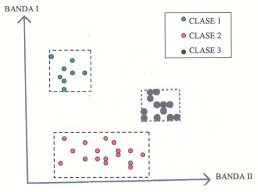
\includegraphics[scale=0.85]{./images/clasificacion_supervisada1.jpg}
	\caption{ Ejemplo de un diagrama de dispersi\'on para tres clases.\\ Imagen obtenida del sitio: \emph{ www.teledet.com.uy/tutorial-imagenes-satelitales/clasificacion-supervisada.htm} }
\end{figure}


\newpage
\subsection{Etapa de pruebas}
La etapa de pruebas se debe realizar con elementos que no pertenezcan a los conjuntos de datos etiquetados que se utilizaron en la etapa de entrenamiento, esto para que el resultado sea justamente una prueba del algoritmo y la implementaci\'on ya que, de utilizarse un elemento perteneciente al conjunto de datos etiquetados para una clase en espec\'ifico arrojar\'ia un resultado esperado.\\
Para obtener la clasificaci\'on se utiliza el m\'etodo por el vecino m\'as cercano. Este m\'etodo consiste en obtener la distancia euclidiana, utilizando la Ecuaci\'on (1) entre el elemento de prueba con cada una de las tres clases.

\begin{equation}
	d = \sqrt{ (R_p - R_{in} )^2 + (G_p - G_{in})^2 + (B_p - B_{in})^2 } \\
\end{equation}

Donde:\\
\begin{itemize}
	\item $R_p$, $G_p$ y $B_p$ $\rightarrow$ son los promedios de los canales Rojo, Verde y Azul respectivamente, del prototipo para cada clase.
	\item $R_{in}$, $G_{in}$ y $B_{in}$ $\rightarrow$ son los promedios de los canales Rojo, Verde y Azul respectivamente, de la imagen de entrada para las pruebas
	\item $d$ $\rightarrow$ es la distancia entre el elemento nuevo y una de las tres clases.\\\\
\end{itemize}

Y su clasificaci\'on se har\'a con la distancia menor de las tres distancias calculadas ya que es a la clase que m\'as se acerca de acuerdo a sus caracter\'isticas de color. La Figura 2. muestra un ejemplo de esta etapa.

\begin{figure}[h]
	\setlength{\unitlength}{0.0105in}
	\centering
	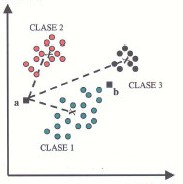
\includegraphics[scale=0.85]{./images/clasificacion_supervisada.jpg}
	\caption{Ejemplo de la etapa de pruebas con un elemento nuevo 'a' para clasificarse con respecto al promedio de color de cada canal para las tres clases.\\ Imagen obtenida del sitio: \emph{ www.teledet.com.uy/tutorial-imagenes-satelitales/clasificacion-supervisada.htm}}
\end{figure}

\newpage
\section{Resultados}
Para realizar el proyecto se plante\'o un escenario donde existiera una banda transpotadora que llevar\'ia a cada pelota hacia una c\'amara a una altura definida que se encargar\'ia de tomar fotos a cada pelota para segmentarlas del fondo y poder obtener las caracter\'istica de color de cada pelota ya sea en la etapa de entrenamiento o en la etapa de pruebas, para despu\'es clasificar la pelota en una de las tres clases que se definieron.\\

El sistema que se implement\'o se muestra en la Figura 3. donde se a\~nadio a la banda transportadora una caja negra lo suficientemente grande para poder controlar las variables f\'isicas como lo son la iluminaci\'on y la distancia entre la c\'amara y el objeto a fotografiar, esto con el fin de que las fotos resultantes no tuviesen alg\'un defecto causado por el ambiente externo.

\begin{figure}[h]
	\setlength{\unitlength}{0.0105in}
	\centering
	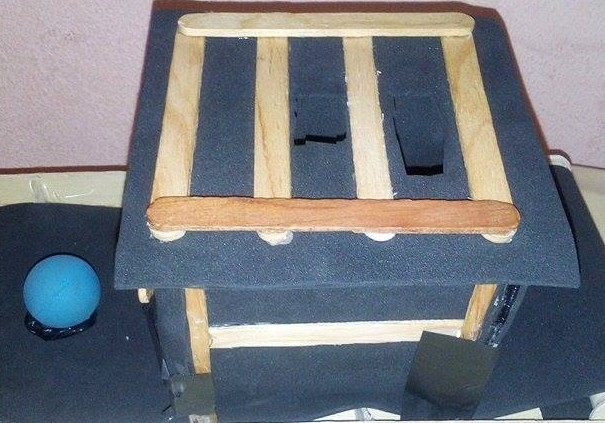
\includegraphics[scale=0.30]{./images/bird_house.jpg}
	\caption{ Caja negra implementada para controlar las variables f\'isicas.}
\end{figure}

Como se puede apreciar en la Figura 3. la caja negra en la parte superior tiene un par de agujero, uno de ellos es para colocar una lampara y el otro es para posar la c\'amara y que pueda captar la imagen dentro de la caja negra con iluminaci\'on controlada. En la Figura 4. se muestra un ejemplo de una foto tomada para una pelota dentro de la caja negra.

\begin{figure}[h]
	\setlength{\unitlength}{0.0105in}
	\centering
	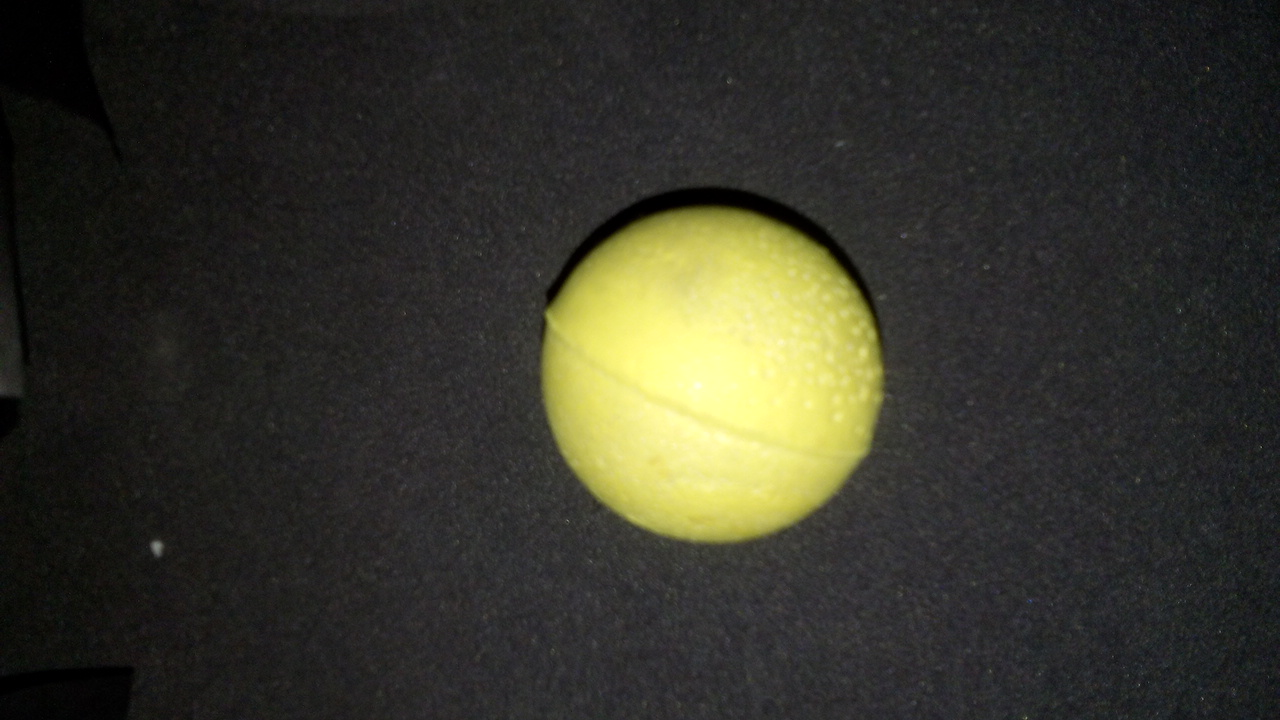
\includegraphics[scale=0.20]{./images/ball_inside.jpg}
	\caption{ Pelota dentro de la caja negra.}	
\end{figure}

Para poder realizar toda la clasificaci\'on primero es necesario segmentar la pelota del fondo. Debido a que el fondo es negro y la pelota resalta facilmente la mejor manera de segmentar la pelota es umbralizando la misma imagen pero en escala de grises, pero no todas las pelotas son del mismo color por lo tanto una umbralizaci\'on con un valor fijo tendr\'a diferentes resultados con pelotas de distintos colores. Para solucionar esto se utiliz\'o un umbral distinto para cada pelota, este umbral es el resultado del m\'etodo de Otsu y al valor que nos da le sumamos $70$ para obtener mejores resultados debido a que se obtienen muchos puntos que no pertenecen al objeto que necesitamos segmentar. El resultado de la umbralizaci\'on para la imagen de la Figura 4. se muestra en la Figura 5. \\

\begin{figure}[h]
	\setlength{\unitlength}{0.0105in}
	\centering
	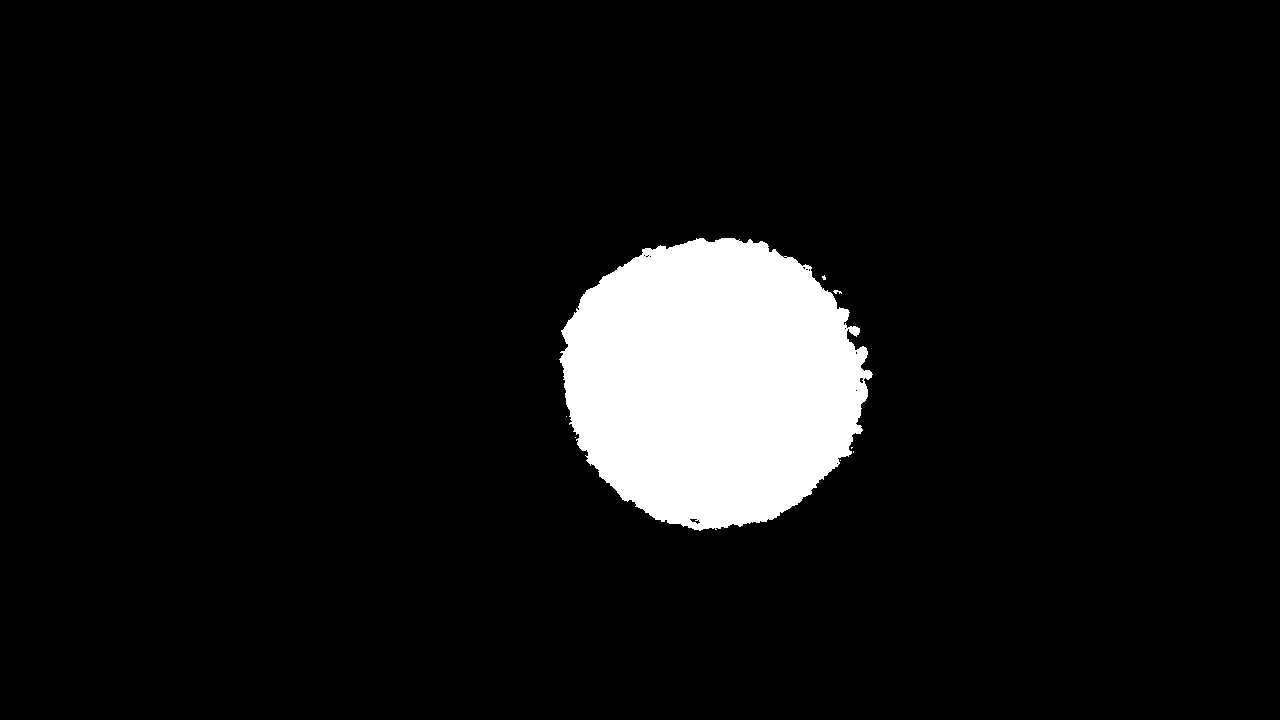
\includegraphics[scale=0.20]{./images/2umbralizacion.png}
	\caption{ Objeto resultante de la umbralizaci\'on con un umbral dado por Otsu al que se le sum\'o $70$.}
\end{figure}

Debido a que a\'un pueden existir objetos o p\'ixeles peque\~nos que no pertenezcan al objeto deseado es necesario eliminarlos de la imagen, esto se logra aplicando morfolog\'ia matem\'atica, en espec\'ifico fue necesario erosionar la imagen con un elemento estructurante en forma de cuadro con dimensiones de $3$ p\'ixeles por lado, esto eliminaba esos objetos no deseados pero tambi\'en afectaba al objeto perteneciente a la pelota, para restaurar un poco su tama\~no y forma es necesario dilatar la imagen con el mismo elemento estructurante. El resultado de estas operaciones se ve en la Figura 6.

\begin{figure}[h]
	\setlength{\unitlength}{0.0105in}
	\centering
	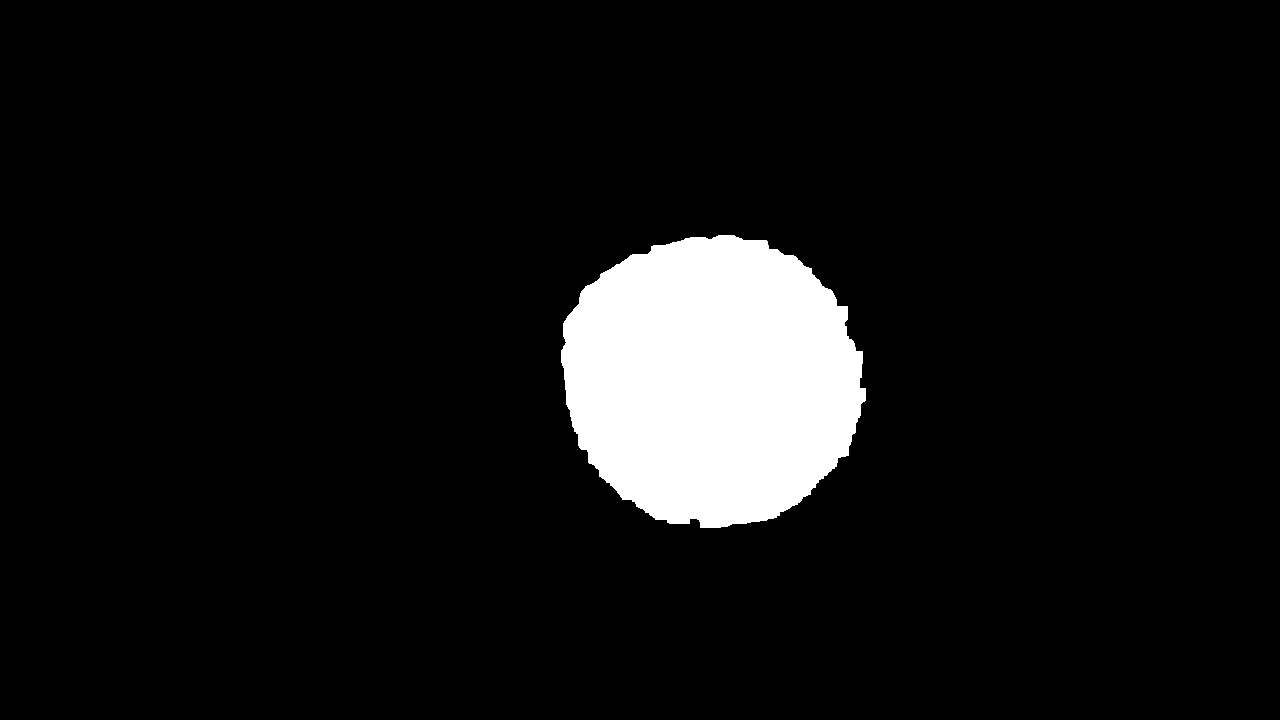
\includegraphics[scale=0.20]{./images/3erosion.png}
	\caption{ Objeto resultante al aplicar morfolog\'ia matem\'atica. }
\end{figure}

Al final es momento de separar el objeto de la imagen de entrada, el resultado se muestra en la Figura 7.

\begin{figure}[h]
	\setlength{\unitlength}{0.0105in}
	\centering
	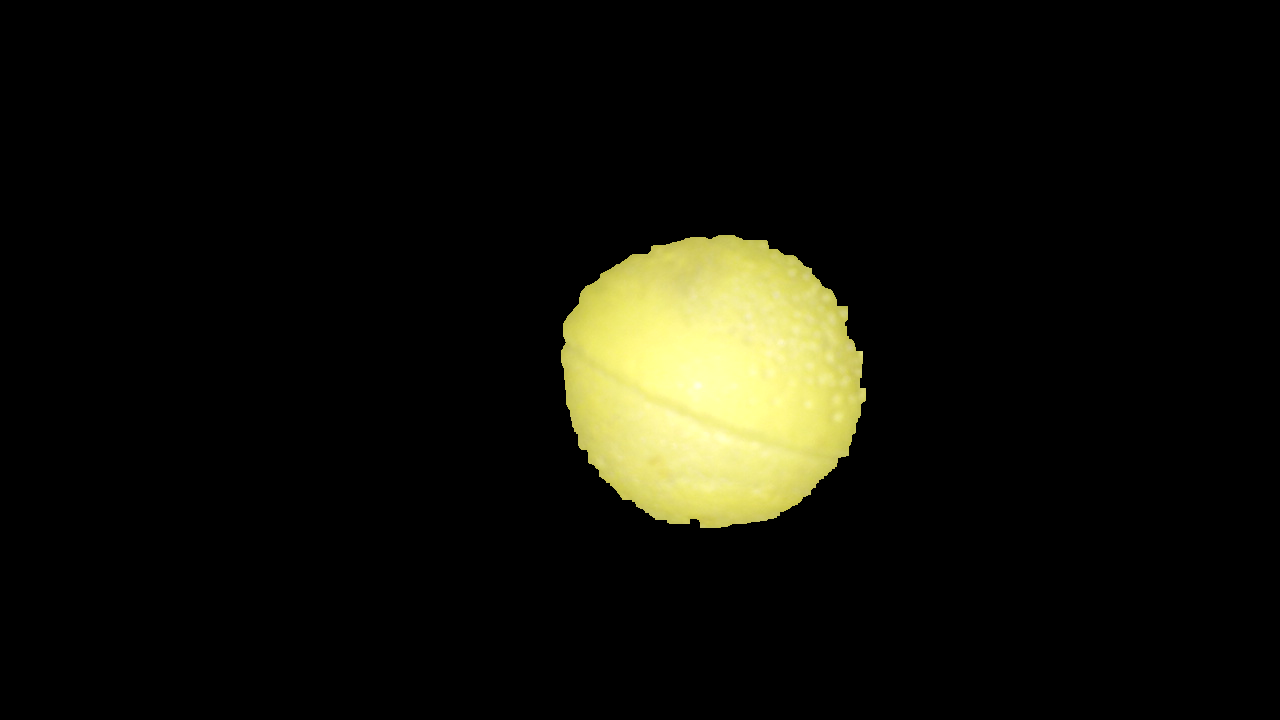
\includegraphics[scale=0.20]{./images/4segmentacion.png}
	\caption{ Pelota segmentada del fondo. }
\end{figure}

Al llegar hasta este punto cualquier pelota se puede segmentar y queda lista para su an\'alisis de las caracter\'isticas de color ya sea para la etapa de entrenamiento o la etapa de pruebas.\\

Se utilizaron tres pelotitas de goma de color Azul, Verde y Rosa (m\'as parecida al rojo) para realizar la etapa de entrenamiento, y un grupo de tres pelotitas de colores Amarillo, Morado y Naranga para realizar la etapa de pruebas. Las pelotitas se muestran en la Figura 8.

\begin{figure}[h]
	\setlength{\unitlength}{0.0105in}
	\centering
	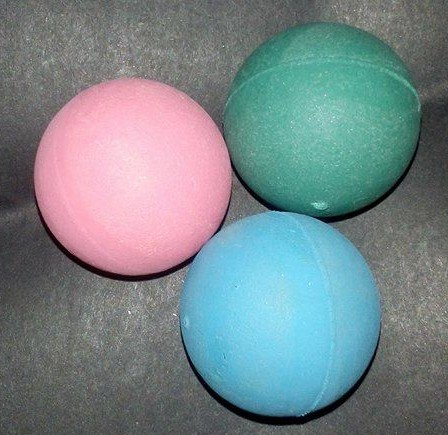
\includegraphics[scale=0.26]{./images/balls1.jpg}
	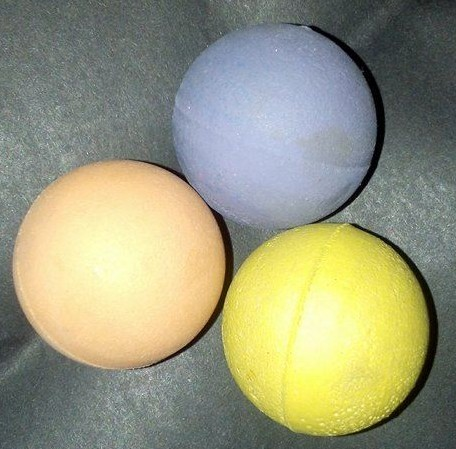
\includegraphics[scale=0.25]{./images/balls2.jpg}
	\caption{ Pelotitas para la etapa de entrenamiento (izquierda) y pelotitas para la etapa de pruebas (derecha). }	
\end{figure}

\newpage
Se definieron tres clases: ClassRed, ClassGreen y ClassBlue. Para obtener los prototipos de cada clase fue necesario obtener el promedio de cada canal de color de $10$ fotos de muestra del mismo objeto en distintas orientaciones para cada uno de los objetos que se consideraron para el entrenamiento. Se utilizaron \'unicamente 3 elementos debido a que no se consiguieron m\'as pelotas y con las que se contaban ten\'ian un color uniforme, por dicha raz\'on s\'olo se tomaron $10$ muestras. Al finalizar la etapa de entrenamiento se obtuvieron los siguientes prototipos para cada clase:\\

\begin{center}
$ClassRed = (255, 225, 230)$ \\
$ClassGreen = (206, 250, 209)$ \\
$ClassBlue = (194, 236, 254)$\\
\end{center}

Y de las cuales se obtuvieron las im\'agenes intermedias mostradas en la Figura 9. como parte de esta etapa de entrenamiento.

\begin{figure}[h]
	\setlength{\unitlength}{0.0105in}
	\centering
	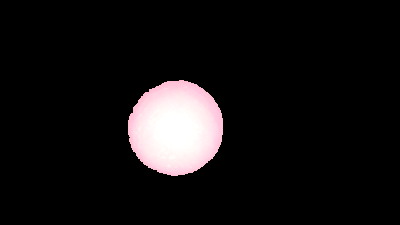
\includegraphics[scale=0.41]{./images/classRed.png}
	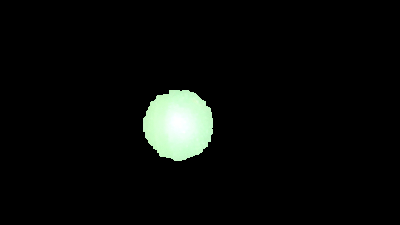
\includegraphics[scale=0.41]{./images/classGreen.png}
	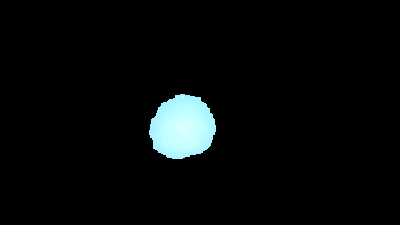
\includegraphics[scale=0.41]{./images/classBlue.png}
	\caption{ Im\'agenes intermedias obtenidas de la fase de entrenamiento para cada una de las clases. }	
\end{figure}

Las etapa de pruebas se realiz\'o con las pelotas de la derecha mostradas en la Figura 8. Como resultado de las pruebas, en la Figura 10 se muestran las im\'agenes intermedias resultantes para las pelotas de prueba.

\begin{figure}[h]
	\setlength{\unitlength}{0.0105in}
	\centering
	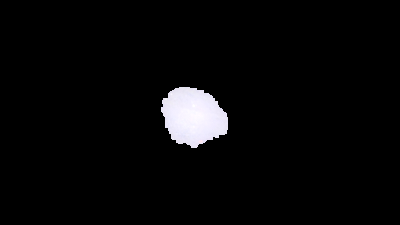
\includegraphics[scale=0.41]{./images/test1.png}
	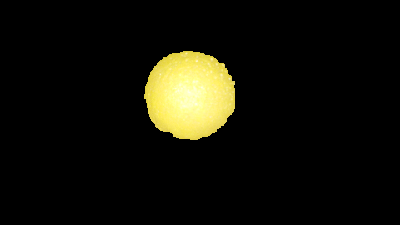
\includegraphics[scale=0.41]{./images/test2.png}
	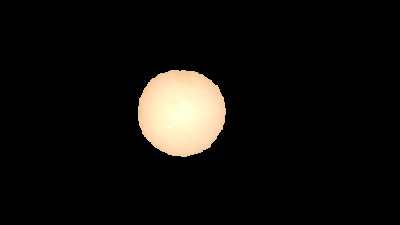
\includegraphics[scale=0.41]{./images/test3.png}
	\caption{ Im\'agenes resultantes de la segmentaci\'on para la etapa de pruebas. Pruebas con las pelotas de color Morado, Amarillo y Anaranjado. }
\end{figure}

\newpage
Por consola se muestran varios datos sobre la clasificaci\'on. En primera, se muestran las distancias que se calcularon de la pelota entrante a cada una de las clases, esto nos da un parametro de medici\'on de la exactitud con que se clasifica la pelota. Otro dato es el promedio de cada canal de la pelota de prueba, esto tambi\'en nos ayuda a calificar si se realiz\'o correctamente tanto la segmentaci\'on y el promediado de los datos como su clasificaci\'on.\\

Los resultados arrojados para la pelota de color Morado se muestran en la Figura 11.
\begin{figure}[h]
	\setlength{\unitlength}{0.0105in}
	\centering
	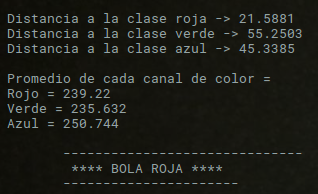
\includegraphics[scale=0.41]{./images/Console1.png}
	\caption{ Datos resultantes de la clasificaci\'on para la pelota color morado. }
\end{figure}

Podemos observar que la pelota fue clasificada como roja, es una sorpresa ya que a primera instancia no se puede apreciar una similitud entre ambos colores pero si observamos el promedio de cada color de la imagen de entrada, correspondiente a la pelota morada, y lo comparamos con el prototipo para la clase ClassRed podemos observar que el valor absoluto de la diferencia entre los promedios es $(15.78, 10.62, 20.74)$ lo que produce que la distancia a esta clase sea la m\'as costa y se clasifique como una pelota Roja. 

\begin{figure}[h]
	\setlength{\unitlength}{0.0105in}
	\centering
	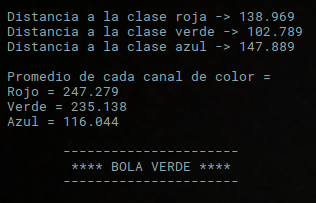
\includegraphics[scale=0.41]{./images/Console2.png}
	\caption{ Datos resultantes de la clasificaci\'on para la pelota color amarillo. }
\end{figure}

\newpage
De acuerdo a la imagen de la Figura 12. para el caso de la pelota color amarillo, \'esta es clasificada como una pelota verde, nuevamente observemos los datos que arroja la consola, mas espec\'ificamente los promedios de cada cada de color de la imagen correspondiente a la pelota amarilla y realizamos el mismo procedimiento que con la pelota morada, obtenemos el valor absoluto de la diferencia entre cada promedio de color, lo que da como resultado $(41.27, 14.86, 92.96)$ y que nos asegura que la distancia era m\'inima entre las caracter\'isticas de color de la imagen de entrada y la clase ClassGreen.

\begin{figure}[h]
	\setlength{\unitlength}{0.0105in}
	\centering
	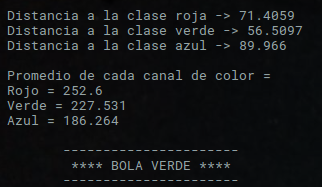
\includegraphics[scale=0.41]{./images/Console3.png}
	\caption{ Datos resultantes de la clasificaci\'on para la pelota color anaranjado. }
\end{figure}

Como podemos observar en la Figura 13. nos arroja los resultados tanto de clasificaci\'on como de promedios y distancias. Con estos datos y siguiendo el mismo procedimiento podemos obtener el valor absoluto de las diferencias entre cada promedio de colores, lo que resulta $(46.6, 22.47, 22.74)$ y nos ayuda a comprobar el resultado de la clasificaci\'on como pelota verde.

\newpage
\section{Conclusiones}
EL proyecto en un inicio pretendia implementarse en una banda transportadora en movimiento y con un sistema de control que estuviese conectado y realizando acciones de acuerdo a los resultados arrojados por el algoritmo de segmentaci\'on, esto no se pudo realizar debido a que surgieron errores al momento de implementar la transformada de Hough para detectar c\'irculos, estos errores consumieron mucho tiempo adem\'as de que su implementaci\'on era muy tardada. Con estos errores se fue consumiendo el tiempo y la parte electr\'onica encargada del control no se implement\'o y se di\'o prioridad a la programaci\'on del algoritmo para segmentar la pelota del fondo y el propio algoritmo para la clasificaci\'on.\\

Hay muchos aspectos a mejorar, entre los que se incluyen mejorar el sistema para la obtenci\'on de im\'agenes, tanto la caja negra como la iluminaci\'on. Otro aspecto a mejorar es aumentar el n\'umero de clases y realizar la etapa de entrenamiento con un n\'umero m\'as variado y suficiente de muestras y de igual manera la etapa de pruebas. Lo anterior para poder clasificar una mayor cantidad de pelotas y obtener un mayor grado de exatitud al clasificar.\\

%$\begin{bmatrix}
% 1 & 1 & 1 & 1 \\
% 1 & 1 & 1 & 1 \\
% 1 & 1 & 1 & 1 \\
% 1 & 1 & 1 & 1 \\
%\end{bmatrix}$

%\begin{thebibliography}{1}
%    \bibitem{IEEEhowto:kopka}
%    H.~Kopka and P.~W. Daly, \emph{A Guide to \LaTeX}, 3rd~ed.\hskip 1em plus
%      0.5em minus 0.4em\relax Harlow, England: Addison-Wesley, 1999.
%\end{thebibliography}

\end{document}
